\citeauthor{Tukey1977} introduced and promoted the term of \ac{EDA} in 1977 to encourage statisticians to explore data and possibly formulate hypotheses that could lead to new data collection and experiments. Many \ac{EDA} ideas can be traced back to earlier authors, but \citeauthor{Tukey1977} summarised all of those ideas with the introduced term. Even though the earlier ideas have all been in combination with statistics, \citeauthor{Tukey1977} encouraged the research field of statistics to use the capabilities of dynamic visualisations in combination with given data. Before that encouragement, statisticians had a strong focus on statistical hypothesis testing without any visualisation. This development supported the identification of outliers, trends and patterns in data in a visual and understandable way \iacite{Tukey1977}. Thus it is possible to derive objectives of \ac{EDA} as follows \iacite{Behrens1997}:

\begin{itemize}

\item Suggest hypotheses about the causes of observed phenomena.
\item Assess assumptions on which statistical inference will be based
\item Support the selection of appropriate statistical tools and techniques
\item Provide a basis for further data collection through surveys or experiments.

\end{itemize}

As of today, there are a number of techniques assisting the field of \ac{EDA}, but the field is more characterised by the attitude taken than by particular techniques \iacite{Tukey1980}. Typical graphical techniques used in \ac{EDA} are box plots, histograms, scatter plots, stem-and-leaf plots, and so forth. This section only discusses histograms in detail.

\citeauthor{Pearson1895} introduced histograms as a graphical representation of the distribution of numerical data. It is an estimate of the probability distribution of a quantitative variable \iacite{Pearson1895}. As the history of visualisation shows (see Chapter \ref{s:history} on page \pageref{s:history} for more detail), cartography also had the goal to visualise distributions on thematic maps. It especially emphasised a spatial variation of one or a small number of geographic distributions.

However, it is needed to consider the task of a user accomplished with the help of a visualisation, as already discussed in Chapter \ref{s:basics} on page \pageref{s:basics}. If a visualisation is not used by the creator and therefore does not fulfill the task of exploring unknown data and deriving new knowledge, it is used to present the given data in some way. A visualisation created for presentation is limited in the kinds of data and tasks it can address. Addressing such a task with a visualisation does not require the user to have domain knowledge. The cruical point of presenting information is that the underlying data is already understood by the creator and the visualisation was created to present the results to an audience \iacite{Munzner2014}.

With this in mind, this chapter could be taken to subsume the two main foci of the thesis: statistical graphics and thematic cartography. Both of these are concerned with graphical representations of quantitative and categorical data but driven by different representational goals. \citeauthor{Friendly.2001} describes the objectives of cartographic visualisation as ``finding the representation constrained to a spatial domain'' whereas statistical graphics try to apply to any domain in the service of statistical analysis \iacite{Friendly.2001}. In addition, cartography and statistical graphics share the common goals of visual representation for exploration and discovery. These range from the simple mapping of locations (land mass, rivers, terrain), to spatial distributions of geographic characteristics (species, disease, ecosystems), to the wide variety of graphic methods used to portray patterns, trends, and indications \iacite{Friendly.2001}. The combination of analytical reasoning with visual representations lead to the research field of visual analytics.

According to \citeauthor{Keim2010}, visual analytics ``[\ldots] is not easy to define, due to its multi-disciplinary nature involving multiple processes and the wide variety of application areas'' \iacite{Keim2010}. Based on current practice, they define visual analytics as the combination of automated analysis techniques with interactive visualisations for an effective understanding, reasoning and decision-making on the basis of very large and complex datasets \iacite{Keim2010}.

So, based on the definition, \citeauthor{Keim2010} elaborate the objectives of visual analytics to state that it is the creation of tools and techniques to enable people to:

\begin{itemize}
\item Summarise information and derive insight from heterogeneous and often conflicting data
\item Detect the expected and discover the unexpected
\item Provide reasonable and understandable evaluations
\item Communicate these evaluations effectively for action
\end{itemize}

\newpage
The following part of this section gives an overview of how visual analytics tries to achieve these objectives to generate knowledge from data. Based upon the knowledge gathered in this section and the sections before, it is possible to derive design principles for good visualisations.

Figure \ref{fig:va-process} on page \pageref{fig:va-process} shows an abstract overview of the visual analytics process. It contains different stages, represented as colored ovals, and their corresponding transitions, represented as arrows. The first step of the process deals with the integration of heterogeneous data sources. This integration includes tasks like data preprocessing, transforming, cleaning, normalisation, grouping, and fusion. All those tasks are indicated by the transformation transition onto the data oval. After the transformation, the analyst has two different options to choose \iacite{Keim2010}:

\begin{enumerate}
\ditem{Automated data analysis} \hfill \\
If an automated model was chosen first, data mining methods are applied to generate statistical models out of the original data. Once the model is made, the analyst only needs to refine its parameters and evaluate it afterwards. The advantage of this choice is the scalability because it can be fully automatised. This automatisation is also the main disadvantage. The model runs in a black box fashion, ignoring all interactions. If this is done, the evaluation of the model can be accomplished with a visualisation. This makes it possible to interact with the data later on \iacite{Keim2010}.

\ditem{Visual data exploration} \hfill \\
If visual data exploration is chosen first, interaction with the generated visualisation is needed to construct insightful information. Interaction could be integrated by zooming or considering different views on the data. Findings can be used to create automatic models. The main advantage of this approach is the interaction with an analyst, thus offering more flexibility and possibilities. On the other hand, it is not scaleable in any way.
\end{enumerate}

\begin{figure}[!htb]
    \centering
    \subcaptionbox
    [
        The visual analytics process is characterised through interaction between data, visualisations, models about the data and the users in order to discover knowledge \iacite{Keim2010}.
    ]
    {
        The visual analytics process is characterised through interaction between data, visualisations, models about the data and the users in order to discover knowledge.
        \label{fig:va-process}
    }
  [0.45\linewidth]
    {
        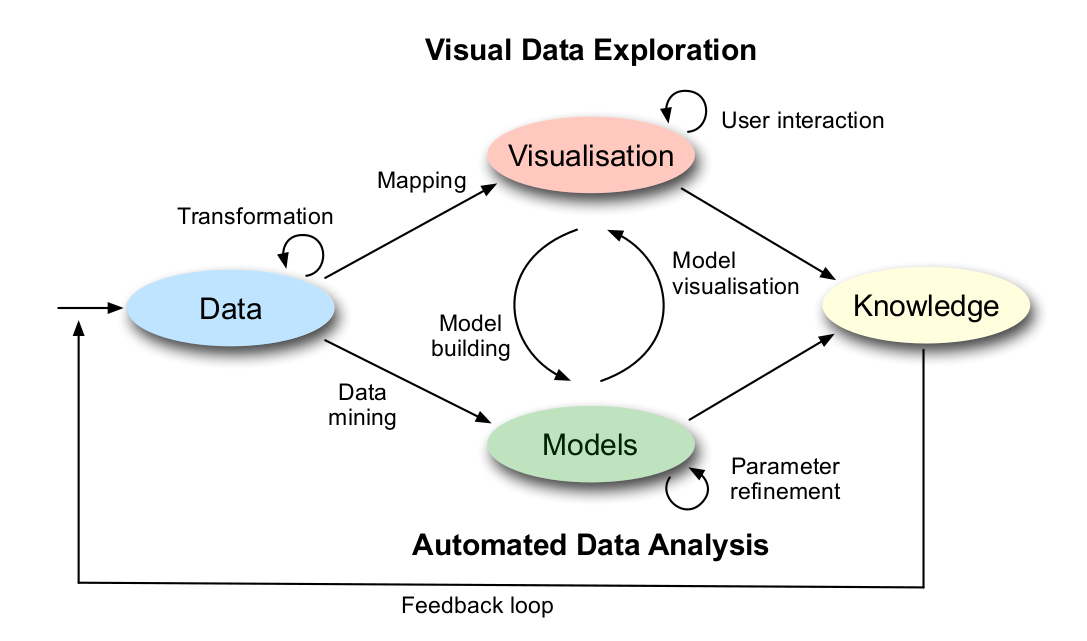
\includegraphics[width=0.5\textwidth,keepaspectratio]
        {images/va/va-process.png}
    }
    \qquad
    \subcaptionbox
    [
        Visual analytics with core adjacent disciplines \iacite{Keim2010}.
    ]
    {
        Visual analytics with core adjacent disciplines.
        \label{fig:va-related}
    }
    [0.45\linewidth]
    {
        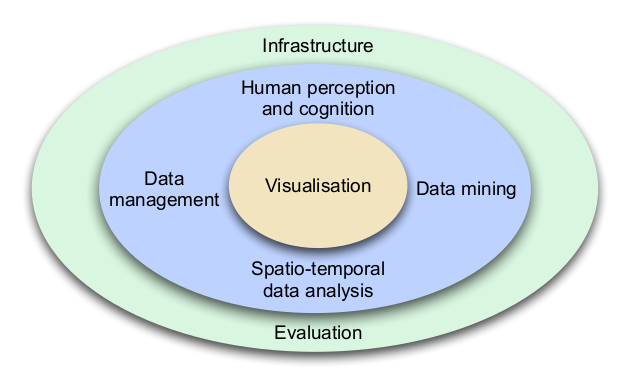
\includegraphics[width=0.4\textwidth,keepaspectratio]
        {images/va/va-related.png}
    }

    \caption{The visual analytics process with its core adjacent disciplines.}
\end{figure}

If automated data and visual data analysis are used in an agile way like iterating both analysis methods in sequence until knowledge is discovered, misleading results in an intermediate step can be discovered and eliminated at an early stage and thus leading to higher confidence and better results \iacite{Keim2010}.

In summary, it can be said that the visual analytics process extracts knowledge gained from visualisations, automatised analysis, and a human analyst combining these two.

Figure \ref{fig:va-related} on page \pageref{fig:va-related} shows the interdisciplinary character of visual analytics. With visualisation as its core, other disciplines like data management, data analysis, and data mining are close related and seem kind of obvious based on the knowledge of the visual analytics process and the definition of the term itself.
